\documentclass[12pt,letterpaper]{article}

\def\myauthor{Juno~Woods}
\def\mytitle{jow-vita}
\def\myemail{juno@translunar.io}
\def\myweb{translunar}
\def\myphone{703-801-2625}
\def\mykeywords{
  juno woods,
  juno september woods,
  juno s woods,
  resume, 
  curriculum, 
  vita, 
  curriculum vita, 
  cv, 
  woods,
  linear covariance analysis,
  lincov,
  ekf,
  extended kalman filter,
  kalman filter,
  candidate optimal groups,
  cog,
  state estimation,
  gn\&c,
  navigation,
  control,
  guidance,
  powered explicit guidance,
  orbit determination,
  batch least squares,
  batch estimator,
  sequential filter,
  navigation filter,
  LunaNet,
  trajectory optimization,
  mission design,
  export control,
  open source,
  patched conic,
  cr3bp,
  trajectory design,
  space policy,
  bioinformatics,
  systems biology,
  synthetic biology,
  personalized medicine,
  computational biology
  automation,
  control systems,
  PID controllers,
  finite state automata,
  state machines,
  programmable logic controllers,
  expert recommendation systems,
  expert recommendation,
  machine learning,
  natural language processing,
  NLP,
  computer vision,
  CV,
  OpenCV,
  zeromq,
  0mq,
  large language models,
  LLMs,
  ChatGPT,
  Claude,
  Anthropic,
  OpenAI,
  PyTorch
}

\setlength\parindent{0pt}

\newenvironment{itemize*}%
{\begin{itemize}%
  \setlength{\itemsep}{0pt}}%
{\end{itemize}}

\usepackage{cfr-lm}
\usepackage{graphicx}
\usepackage{wrapfig}
\usepackage{pgfplots}
\usepackage{amsmath}
\usepackage{textcomp}
\usepackage{url}
\usepackage{fancyhdr}
\usepackage{amssymb}
%\headheight 15ptz
\usepackage{lastpage}
%\usepackage{ocgtools}
\usepackage{enumitem}
\setlist{nolistsep,leftmargin=0.15in}
\usepackage[log-declarations=false]{xparse}
%\usepackage{mathdesign}
%\usepackage[no-math]{fontspec}
\usepackage{microtype}
\usepackage{bold-extra}
\usepackage[margin=1.125in,top=1.375in,right=1in,left=2in]{geometry}
\usepackage[strict]{changepage}
\usepackage[
  ocgcolorlinks,
  urlcolor={[rgb]{0,0,0.54}},
  unicode,
  plainpages=false,
  pdfpagelabels,
  pdftitle={\mytitle},
  pdfauthor={\myauthor},
  pdfkeywords={\mykeywords}
]{hyperref}
\usepackage{relsize}

% Use sans serif fonts in plot
\usepackage[eulergreek]{sansmath}
\pgfplotsset{
  every axis/.append style = {font=\sansmath\sffamily},
  %every axis label = {font=\sansmath\sffamily},
  %legend style = {font=\sansmath\sffamily},
  %tick label style = {font=\sansmath\sffamily},
  %every node style = {font=\sansmath\sffamily}
  }

% fix ocgcolor link breaking; thanks due to Benjamin Lerner (http://goo.gl/VZKR7M)
\makeatletter
\AtBeginDocument{%
  \newlength{\temp@x}%
  \newlength{\temp@y}%
  \newlength{\temp@w}%
  \newlength{\temp@h}%
  \def\my@coords#1#2#3#4{%
    \setlength{\temp@x}{#1}%
    \setlength{\temp@y}{#2}%
    \setlength{\temp@w}{#3}%
    \setlength{\temp@h}{#4}%
    \adjustlengths{}%
    \my@pdfliteral{\strip@pt\temp@x\space\strip@pt\temp@y\space\strip@pt\temp@w\space\strip@pt\temp@h\space re}}%
  \ifpdf
    \typeout{In PDF mode}%
    \def\my@pdfliteral#1{\pdfliteral page{#1}}% I don't know why % this command...
    \def\adjustlengths{}%
  \fi
  \ifxetex
    \def\my@pdfliteral #1{\special{pdf: literal direct #1}}% isn't equivalent to this one
    \def\adjustlengths{\setlength{\temp@h}{-\temp@h}\addtolength{\temp@y}{1in}\addtolength{\temp@x}{-1in}}%
  \fi%
  \def\Hy@colorlink#1{%
    \begingroup
      \ifHy@ocgcolorlinks
        \def\Hy@ocgcolor{#1}%
        \my@pdfliteral{q}%
        \my@pdfliteral{7 Tr}% Set text mode to clipping-only
      \else
        \HyColor@UseColor#1%
      \fi
  }%
  \def\Hy@endcolorlink{%
    \ifHy@ocgcolorlinks%
      \my@pdfliteral{/OC/OCPrint BDC}%
      \my@coords{0pt}{0pt}{\pdfpagewidth}{\pdfpageheight}%
      \my@pdfliteral{F}% Fill clipping path (the url's text) with current color
      \my@pdfliteral{EMC/OC/OCView BDC}%
      \begingroup%
        \expandafter\HyColor@UseColor\Hy@ocgcolor%
        \my@coords{0pt}{0pt}{\pdfpagewidth}{\pdfpageheight}%
        \my@pdfliteral{F}% Fill clipping path (the url's text) with \Hy@ocgcolor
      \endgroup%
      \my@pdfliteral{EMC}%
      \my@pdfliteral{0 Tr}% Reset text to normal mode
      \my@pdfliteral{Q}%
    \fi
    \endgroup
  }%
}
\makeatother
% end fixes


\newcommand{\Cpp}{\textsc{c}\nolinebreak[4]\hspace{-.05em}\raisebox{.4ex}{\relsize{-3}{\textbf{++}}}}
\newcommand{\Magickpp}{Magick\nolinebreak[4]\hspace{-.05em}\raisebox{.4ex}{\relsize{-3}{\textbf{++}}}}
\newcommand{\Star}{\textsc{Star-CCM\ensuremath{+}}}

\newcommand{\mhead}[1]{\leavevmode\marginpar{\sffamily\footnotesize #1}}
%\newcommand{\rdate}[1]{{\addfontfeature{Numbers=OldStyle} \hfill #1}}
%\renewcommand{\date}[1]{{\addfontfeature{Numbers=OldStyle} #1}}
\newcommand{\rdate}[1]{{\hfill #1}}
\renewcommand{\date}[1]{{#1}}
\renewcommand{\labelitemi}{-}

%\setmainfont[
%  Ligatures={TeX,Common},
%  BoldFont={AGaramondPro-Semibold},
%]{Adobe Garamond Pro}
%\setsansfont[
%  Ligatures={TeX,Common},
%  Letters=SmallCaps,
%  Color=660000,
%]{Adobe Garamond Pro}
%\setmonofont[Scale=0.85]{FontAwesome}

%\makeatletter % fix for \hrulefill w/ mathdesign package
%\def\hrulefill{\leavevmode\leaders \hrule height \rulethickness \hfill\kern\z@}
%\makeatletter

\begin{document}\flushbottom
\pagestyle{fancy} \setlength\headwidth{6.5in}
\rhead{\textsc{Dr.~Juno~Woods --- curriculum vitae --- \thepage{} of \pageref*{LastPage}}} \cfoot{}
\thispagestyle{empty}
\begin{adjustwidth}{-1in}{}
{\Huge
  {\textsc{%
    %{%\addfontfeature{Style=TitlingCaps}
    %J}\kern-1.0ptohn 
    %{%\addfontfeature{Style=TitlingCaps}
    %O}\kern-2pt.~``%
    {%\addfontfeature{Style=TitlingCaps}
    J}\kern-2ptuno~%
    {%\addfontfeature{Style=TitlingCaps}
    W}\kern-2.5ptoods, PhD}
  }
  }
%
{
  \begin{minipage}[b]{1.3in}
    \flushleft \footnotesize   
    \href{tel:\myphone}{\myphone} \\ %\texttt{}~
    \href{mailto:\myemail}{\myemail}
  \end{minipage}
  \hfill
  \begin{minipage}[b]{1.3in}
    \flushright \footnotesize 
    github:\href{https://github.com/translunar}{translunar} \\
    linkedin:\href{https://www.linkedin.com/in/translunar}{translunar}
  \end{minipage}
}\par
\hrulefill

\centering\small Original mission designer for Odysseus (\textsc{im}-1), the first private lunar lander on the Moon.
\vskip-6pt
\hrulefill
\end{adjustwidth}
\reversemarginpar 
\setlength\marginparwidth{0.85in}
\smallskip

\mhead{Education}%
\textbf{The University of Texas at Austin,} Austin, Texas \newline
\emph{Doctor of Philosophy, Cell \& Molecular Biology (Bioinformatics)}\rdate{2007--2013}
\begin{itemize*}
  \item National Science Foundation Fellow (2009--2012), \href{http://cssb.utexas.edu/}{Center for Systems \& Synthetic Biology} % 3.7646 GPA
 %\item Dissertation: \href{https://www.dropbox.com/s/87v8j47mxo0afgj/diss.pdf}{Predicting gene--phenotype associations in humans and other species from orthologous and paralogous phenotypes}
  \item Advisor: Dr.~Edward~M.~Marcotte
\end{itemize*}

\medskip
\textbf{Virginia Polytechnic Institute \& State University,} Blacksburg, Virginia \newline
\emph{Bachelor of Science, Computer Science}, magna cum laude \rdate{2002--2007}
\begin{itemize*}
  %\item Graduated \emph{magna cum laude} % 3.66 GPA
  \item Minors in Mathematics, Philosophy, and Russian
\end{itemize*}

\bigskip
\mhead{Professional \newline Appointments}%
\vskip -1em
\textbf{Astranis,} San Francisco, California \newline
\emph{Senior \textsc{gn\&c} engineer \textsc{ii}} \rdate{\textsc{apr}~2024--\textsc{present}}
%\begin{itemize*}
%    \item 
%\end{itemize*}

\medskip
\textbf{Charm Industrial,} San Francisco, California \newline
\emph{Senior software engineer, control systems} \rdate{\textsc{oct}~2022--\textsc{may}~2023}
\begin{itemize*}
    \item Designed, implemented, and hardware-in-the-loop tested custom process automation framework (finite state automata and various \textsc{pid} controllers) for use in carbon sequestration
    \item Implemented continuous integration workflows (software integration and build management), contributed to software process and procedure development
    %\item Wrote plant models for chemical engineering processes in fast pyrolysis-based carbon sequestration
\end{itemize*}
%
\medskip
\textbf{Masten Space Systems,} Mojave, California \newline
\emph{\textsc{gn\&c} engineer, 6-\textsc{dof} (contractor)} \rdate{\textsc{jul}~2021--\textsc{jun}~2022}
\begin{itemize*}
   %\item Derived and wrote simulation sensor models, designed Monte Carlo simulation configurations
   \item Derived, designed, and prototyped navigation system (\textsc{ekf}) and simulation configuration for \textsc{xl}-1 lunar lander
   %\item Performed guidance algorithm trade, derived powered explicit guidance laws
   \item Designed flight manager for high-level planning of \textsc{gn\&c} activities
%   \item Derived, designed, and prototyped linear algebra models (\textsc{ekf}) for integrating sensor data into time series least squares model, including attitude
\end{itemize*}
%
%\medskip
%\textbf{Charismatic Metafauna by Majorelle Arts,} Oakland, California \newline
%\emph{Concept designer} \rdate{2021--2022}
%\begin{itemize*}
%   \item Proposed (and built) Burning Man honorarium project: When participants interact negatively with these metal sculptures of endangered species, as observed by neural network, the fire inside them dims and the music changes; when participants play music to the animals, their virtual `health' improves and they sing back to the participants
%   \item Coordinating activities of sound design team and interfacing with interactivity team to fulfill engineering requirements
%\end{itemize*}
%

%\medskip
%\textbf{Numina Studios / Nocturne-X,} Oakland, California \newline
%\emph{Electronics Assembly (contractor)} \rdate{\textsc{sep}--\textsc{oct}~2021}
%\begin{itemize*}
%   \item Soldering and electronics assembly for a large-budget interactive art experience at Gray Area in San Francisco for three months beginning October~2021
%\end{itemize*}
%
%\medskip
%\textbf{Metalunar, \textsc{\textbf{llc}}}, Boulder, Colorado / \textbf{Translunar, \textsc{\textbf{llc}}}, Berkeley, California \newline
%\emph{Co-founder} \rdate{\textsc{apr}~2020--\textsc{present}}
%\begin{itemize*}
%  \item Systems engineering: \textsc{gn\&c} systems, optical navigation, and interplanetary radios (LunaNet)
%  \item Business models (system requirements, budget, timeline, market analysis) 
%  \item Proposal writing
%\end{itemize*}

\medskip
\textbf{Open Lunar Foundation,} San Francisco, California \newline
%\begin{itemize*}
%  \item Worked with small team to develop strategy for a space industry non-profit focused on lunar settlement
%  \item Analyzed 
%  \item Created business plans, engineering schedules, and financial models for various for-profit interventions
%\end{itemize*}
\emph{Senior Researcher} \rdate{\textsc{mar}--\textsc{jul}~2021} \\
\emph{Director of Engineering Research \& Strategy} \rdate{\textsc{jul}~2020--\textsc{mar}~2021} \\
\emph{Guidance, Navigation, \& Control} \rdate{\textsc{oct}~2019--\textsc{apr}~2020}
\begin{itemize*}
  %\item Managed multiple research fellows to deliver trajectory designs, business plans, and technical reports 
  \item Designs and analyses: navigation, orbit determination, sensors, trajectory, terrain-relative navigation (computer vision and image processing using shape from shading, structure from motion), open source tool for linear covariance analysis, \textsc{imu} selection trade
  %\item Space policy: multilateral arms control treaties, export control policy, open source, electronic frontiers
  \item Systems engineering: \textsc{gn\&c} systems, optical navigation, and interplanetary radios
\end{itemize*}

\medskip
\textbf{Intuitive Machines,} Houston, Texas \newline
\emph{Senior Development Engineer} \rdate{\textsc{jun}~2015--\textsc{sep}~2019} % June 22 - Sep 27
\begin{itemize*}
  \item Original mission designer for \textsc{nova-c}, the first private lunar lander on the surface of the Moon: trajectory design, camera placements and specifications, attitude timeline, ground station selection, \textsc{imu} specifications, linear covariance analysis
  \item Derived sensor models, including: \textsc{gps}, attitude, bearing, altimetry, navigation Doppler \textsc{lidar} (velocimetry)
  \item Worked on hardware-in-the-loop and software simulations, wrote multiple state estimation systems (batch least squares, complementary filters, extended Kalman filters) during design phase across two lunar landers, a commercial space station, and several drilling projects
  \item Experience in inertial and local coordinate systems
  % \item Simulation models and configurations in Trick, worked with Core Flight Software
  \item Cislunar communications architecture analyses for a satellite constellation
\end{itemize*}

\bigskip
\mhead{Academic \newline Appointments}%
\textbf{Applied Space Exploration Laboratory,} West Virginia University \newline
\emph{Post-doctoral Fellow --- Aerospace Engineer} \rdate{\textsc{jan}~2014--\textsc{jun}~2015}
\begin{itemize*}
  \item Assisted with management, coordination, and mentoring of graduate students working with low-cost \textsc{imu} swarms
  \item \textsc{Lidar}-based strategy for non-cooperative rendezvous for satellite servicing and asteroid rendezvous, including 6-\textsc{dof} dynamics simulation, including point cloud image processing algorithms
  \item Open source Open\textsc{gl}-based \textsc{3d} sensor simulator, \textsc{Glidar}
  \item Remote sensing technologies for resource surveying and utilization
\end{itemize*}

\medskip
\textbf{Center for Systems \& Synthetic Biology,} The University of Texas at Austin\newline
\emph{National Science Foundation Fellow; Graduate Research Assistant}  \rdate{2007--2014}
\begin{itemize*}
  \item Mentored other undergraduate and graduate students
  % \item Pipelines and automation for large datasets; expert recommendation systems, cross-validation
  \item Wrote numerical methods and linear algebra toolkit for the Ruby language
  %\item Statistical software for searching for genes under various types of selection (positive, purifying, relaxed)
  %\item Viral evolution simulation for understanding \textsc{hiv} reservoirs
  %\item Scheme and partial implementation re-engineering cellular metabolism in \textit{E.~coli}
\end{itemize*}

\medskip
\textbf{Dept. of Chemistry \& Biochemistry,} The University of Texas at Austin\newline
\emph{Graduate Teaching Assistant} \rdate{2008, 2013}
\begin{itemize*}
%  \item Served as \textsc{ta} for Biochemistry, Introduction to Bioinformatics (graduate level), and Chemistry for non-science majors
  \item Rewrote curriculum for Introduction to Bioinformatics in Python (previously in Perl) %, largely focused on string processing and search algorithms, hidden Markov models, etc.
\end{itemize*}

\medskip
\textbf{Dept. of Computer Science,} Virginia Tech\newline
\emph{Undergraduate Research Assistant} \rdate{Summer 2006}
\begin{itemize*}
  \item Noun phrase extraction from abstracts for concept map generation (natural language processing)
\end{itemize*}

\bigskip
\mhead{Community Contributions}
\vskip -1em

\medskip
\textbf{Texas Gun Sense,} Austin, Texas \newline
\emph{Co-founder} \rdate{2008--\textsc{jul}~2013}
\begin{itemize*}
   \item Co-founded a non-profit providing evidence-based public safety recommendations to the public in Texas
\end{itemize*}
%  \item Provided first-hand expertise in mass casualty situations
%  \item Served as student appointee to the University of Texas System Police Academy Advisory Board
%  \item Evidence-based public safety policy analyses related to firearms aimed toward the Texas Legislature
%  \item Statistical analyses on public health and crime information
%\end{itemize*}

%\textbf{Take 3 Presents}\newline
%\emph{Greeters Lead} \rdate{\textsc{Mar} 2022--\textsc{present}}
%\begin{itemize*}
%  \item Have written and proposed multiple budgets, hired team members
%  \item Management of one employee and a team of volunteers to deliver a project within budget and on time
%  \item Onboarding new participants so they understand responsibilities in an interactive theater container, prioritizing consent, participation, and responsibility
%\end{itemize*}

\medskip
\textbf{Black Rock Rangers}\rdate{2018--\textsc{present}}\newline
\emph{Green Dot} \rdate{2019--\textsc{present}} \newline
\emph{Green Dot Trainer} \rdate{\textsc{Jun}~2023--\textsc{present}}
\begin{itemize*}
  \item Mental health first aid, holding space, conflict mediation, harm reduction; training of other green dot rangers
  \item Support for those experiencing grief, trauma, addiction
\end{itemize*}

\medskip
\textbf{Lunar Surface Innovation Consortium}\rdate{2021--2023}\newline
\emph{Communications Subgroup Lead} \rdate{2021--2022}

\medskip
\textbf{Ruby Science Foundation (SciRuby)} \newline %The Ruby Science Foundation: The SciRuby Project}\newline
\emph{Director \& Co-Founder} \rdate{2012--2018}
\begin{itemize*}
  \item Wrote Ruby linear algebra library, NMatrix
  \item Mentored Google Summer of Code students and organized mentors
\end{itemize*}

%\medskip
%\textbf{Austin Swing Syndicate}\newline
%\emph{At-Large Board Member, Secretary} \rdate{2012--2014}%\newline%
%


%\newpage
\bigskip
\mhead{Patents}%
\par\vspace{-\baselineskip}Marcotte, E.M.; McGary, K.; Wallingford, J.; Park, T.J.; \textbf{Woods,~J.}; Cha,~H.J. 12 August 2012. Orthologous phenotypes and non-obvious human disease models. \textit{U.S.\ Patent Application Publication 2012/0215458 A1}.


\bigskip
%\newpage
\mhead{Articles}%
\par\vspace{-\baselineskip}%\textit{List of non-aerospace articles authored available upon request.}
%\medskip
\par\textbf{Woods, J.}; Christian, J.A. 2016. \textsc{Lidar}-based relative navigation with respect to non-cooperative objects. \textit{Acta Astronautica 126}: pp.\ 298--311.

\medskip
\par\textbf{Woods, J.}; Christian, J.A. 2016. \textsc{Glidar}: An OpenGL-based, real-time, and open source 3\textsc{d} sensor simulator for testing computer vision algorithms. \textit{Journal of Imaging 2}(1).

\medskip
\par\textbf{Woods, J.}; Tien, M.Z.; Marcotte, E.M. April 2015. Interrogating conserved elements of diseases using Boolean combinations of orthologous phenotypes. \textit{BioR$\chi$iv}.

\medskip
\par\textbf{Woods, J.}; Singh-Blom, U.M.; Laurent, J.M.; McGary, K.L.; Marcotte, E.M. January 2013. Prediction of gene--phenotype associations in humans, mice, and plants using phenologs. \textit{BMC Bioinformatics 14}: p.\ 203.

\medskip
\par Singh-Blom, U.M.; Natarajan, N.; Tewari, A.; \textbf{Woods, J.}; Dhillon, I.S.; Marcotte, E.M. January 2013. Prediction and validation of gene--disease associations using methods inspired by social network analyses. \textit{PLoS One 8}(5): e58977.

\medskip
\par McGary, K.L.; Park, T.J.; \textbf{Woods, J.}; Cha, H.J.; Wallingford, J.B.; Marcotte, E.M. April 2010. Systematic discovery of nonobvious human disease models through orthologous phenotypes. \textit{Proceedings of the National Academy of Sciences of the United States of America 107}(14): pp.\ 6544--9.

\medskip
\par Brennan, T.P.; \textbf{Woods, J.}; Sedaghat, A.R.; Siliciano, J.D.; Siliciano, R.F.; Wilke, C.O. September 2009. Analysis of human immunodeficiency virus type 1 viremia and provirus in resting $\textsc{cd4}^{+}$ \textsc{t} cells reveals a novel source of residual viremia in patients on antiretroviral therapy. \textit{Journal of Virology 83}(17): pp.\ 8470--81.

\bigskip
\mhead{Conference \newline Proceedings}%
\par\vspace{-\baselineskip}\textbf{Woods, J.}; Christian, J.A.; Evans, T. February 2015. A \textsc{6-dof} pose initialization strategy for \textsc{lidar}-based non-cooperative navigation. In \textit{38th Annual Guidance \& Control Conference}, Breckenridge, CO.

\medskip
Sell, J.L.; Rhodes, A.; \textbf{Woods, J.}; Christian, J.A.; Evans, T. 2014. Pose performance of LIDAR-based navigation for satellite servicing. In \textit{AIAA/AAS Astrodynamics Specialist Conference}, San Diego, CA.

\bigskip
\mhead{Posters}%
\par\vspace{-\baselineskip}\textbf{Woods, J.}; Singh-Blom, U.M.; Laurent, J.; McGary, K.L.; Marcotte, E.M. 20--25 February 2012. In \textit{Complex Traits: Genomics and Computational Approaches}, Keystone Symposia, Breckenridge, CO.

\medskip
\par \textbf{Woods, J.}; Singh-Blom, U.M.; McGary, K.L.; Marcotte, E.M. 13--16 November 2010. In \textit{From Functional Genomics to Systems Biology},  EMBL Heidelberg, Heidelberg, Germany.

\bigskip
\mhead{Technical \newline Reports}%
\par\vspace{-\baselineskip}\textit{Some internal technical report titles have been altered for external clarity or to maintain client confidentiality.}

\medskip
\par\textbf{Woods, J.} 2023. A call for a quantitative report card for AI bioterrorism threat models. \textit{Lesswrong}.

\medskip
\par\textbf{Woods, J.} 2022. Design trade for the \textsc{xl}-1 autonomous flight manager. \textit{TLI--TM--2022--01}, Translunar \textsc{llc} for Masten Space Systems, Mojave, CA.

\medskip
\par\textbf{Woods, J.} 2022. Navigation filter design for \textsc{xl}-1. \textit{TLI--TM--2021--03}, Translunar \textsc{llc} for Masten Space Systems, Mojave, CA.

\medskip
\par\textbf{Woods, J.} 2021. The downrange constraint in Powered Explicit Guidance. \textit{TLI--TM--2021--02}, Translunar \textsc{llc} for Masten Space Systems, Mojave, CA.

\medskip
\par\textbf{Woods, J.} 2021. Risk of rock encounters at Haworth landing site. \textit{TLI--TM--2021--01}, Translunar \textsc{llc} for Masten Space Systems, Mojave, CA.

\medskip
\par\textbf{Woods, J.}; McMahon, C. 2021. Open source, open standards, and collective invention in the space industry. \textit{OLF--ENG--2021--02}, Open Lunar Foundation, San Francisco, CA.

\medskip
\par\textbf{Woods, J.} 2021. An engineer's history of US and multilateral export controls. \textit{OLF--ENG--2021--01}, Open Lunar Foundation, San Francisco, CA.

\medskip
\par\textbf{Woods, J.} 2020. Concepts in lunar positioning, navigation, and timing. \textit{OLF--GNC--2020--01}, Open Lunar Foundation, San Francisco, CA.

\medskip
\par\textbf{Woods, J.} 2019. Navigation filter design towards a lunar lander. \textit{OLF--GNC--2019--02}, Open Lunar Foundation, San Francisco, CA. \textit{Work in progress, ceased and published early due to pandemic.} \href{https://github.com/openlunar/navmemos/raw/master/filter/filter.pdf}{github.com/openlunar/navmemos/ raw/master/filter/filter.pdf}

\medskip
\par\textbf{Woods, J.} 2019. Two-way range and range-rate observables in a sequential filter. \textit{OLF--GNC--2019--01}, Open Lunar Foundation, San Francisco, CA. \href{https://github.com/openlunar/navmemos/raw/master/radiometric/memo.pdf}{github.com/openlunar/navmemos/raw/master/radiometric/memo.pdf}

\medskip
\par\textbf{Woods, J.} 2018. Observability and sensitivity analyses for attitude estimation using a gimballed gyroscope. \textit{IM--TM--2018--04}, Intuitive Machines, Houston, TX.

\medskip
\par \textbf{Woods, J.} 2018. Position and velocity variance growth during dead reckoning of a drill. \textit{IM--TM--2018--02}, Intuitive Machines, Houston, TX.

\medskip
\par \textbf{Woods, J.} 2018. Derivation of the Doppler \textsc{lidar} measurement model in the inertial and topocentric frames. \textit{IM--TM--2018--01}, Intuitive Machines, Houston, TX.

\medskip
\par Crain, T.C.; \textbf{Woods, J.}; Baine, M.; Moore, J.; Getchius, J.; Ronalds, A.; Stewart, S. 2018. Cislunar navigation architecture study. \textit{IMDM--9}, Intuitive Machines, Houston, TX.

\medskip
\par \textbf{Woods, J.} 2017. A dual \textsc{marg} complementary filter for attitude state estimation while drilling. \textit{IM--TM--2017--04}, Intuitive Machines, Houston, TX.

\medskip
\par \textbf{Woods, J.}; Christian, J.A. 2014. A real-time, software-based \textsc{3d} sensor simulator. ASEL Technical Memorandum: \textit{ASEL--14--005}, West Virginia University, Morgantown, WV.

\medskip
\par Sell, J.; Rhodes, A.; \textbf{Woods, J.}; Christian, J.A. 2014. Theoretical foundations of pose estimation and covariance computation for non-cooperative relative navigation. ASEL Technical Memorandum: \textit{ASEL--14--001}, West Virginia University, Morgantown, WV.

\medskip
\par Natarajan, N.; Singh-Blom, U.M.; Tewari, A.; \textbf{Woods, J.}; Dhillon, I.S.; Marcotte, E.M. 2011. Predicting gene--disease associations using multiple species data. UTCS Technical Report: \textit{TR--11--37}, University of Texas at Austin, Austin, TX.

\bigskip
%\newpage
\mhead{Selected \\ Honors \& \newline Awards}%
%Burning Man Honorarium: \textit{Charismatic Metafauna}				\rdate{2022}\newline
Masten Space Systems: Diversity, Equity, and Inclusion Council member \rdate{2022}\newline
%Paul Harris Fellowship                                              \rdate{2018}\newline
%Necklace Factory / Burning Man Art Award                            \rdate{2016}\newline
White House Champion of Change				\rdate{2014}\newline
National Science Foundation Graduate Research Fellowship			\rdate{2009--2012}\newline
``Best of Austin'' Award: Best Activist	(\emph{The Austin Chronicle})							\rdate{2011}\newline
Scholar, Netroots Nation											\rdate{2011}\newline
Initiate, Friar Society (University of Texas at Austin)				\rdate{2010}\newline
Graduate School Recruitment Fellowship (University of Texas at Austin) \rdate{2007}\newline
Black Belt, Tae Kwon Do (Chung Do Kwan)								\rdate{2006}\newline
Member, Hillcrest Honors Community (Virginia Tech)				\rdate{2003--2007}\newline
Inductee, $\Upsilon\Pi\mathrm{E}$ (Virginia Tech)					\rdate{2006}\newline
Gilbert \& Lucille Seay Scholarship (Virginia Tech)					\rdate{2005}\newline
National Merit Scholarship											\rdate{2002}%\newline

%\bigskip
%\mhead{Media}%
%\par\vspace{-\baselineskip}\textit{Media appearances available upon request.}
%\bigskip
%\mhead{Activities \& \newline Interests}%
%dance (lindy hop and ballet),
%music,
%roller skating,
%circus arts,
%space exploration,
%large-scale interactive art,
%immersive theatre

\newpage
\mhead{Coding \newline Proficiencies}%
\begin{wrapfigure}{R}{2in}
\vspace{-25pt}%
\centering%
%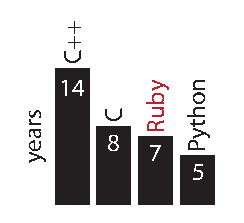
\includegraphics[width=2in]{programming-graph.pdf}%
\begin{tikzpicture}
\begin{axis}[ybar
			, symbolic x coords={C++, C, Ruby, Python, Matlab},
			, ylabel={years}
			, ylabel near ticks
			, ymajorgrids=true
			, axis on top
			, grid style={draw=white, line width=1pt}
			, major tick length=0pt
			, ymin=0
			, xtick=data
			, fill=black
			, fill opacity=1.0
			, draw=white
			, bar width=0.05\textwidth
			, nodes near coords
			, every node near coord/.append style={rotate=90, anchor=west, color=black}
			, width=2in
			, xmajorticks=false
			]
\addplot+[point meta=explicit symbolic,fill=black,draw=white] coordinates {
	(C++,21) [C\footnotesize{++}]
	(C,15) [C]
	(Ruby,10) [Ruby]
	(Python,11) [Python]
	(Matlab,3) [Matlab]
};
\end{axis}
\end{tikzpicture}
\vspace{-15pt}%
\end{wrapfigure}%
%
%\emph{Strong}\ 
\textsc{c},
\Cpp,
Ruby,
Python,
\LaTeX,
\textsc{gnu} Octave / Matlab

\medskip
\emph{Familiar}\ 
Java, \textsc{sql}, shell scripting, Agile

\medskip
\emph{Forgotten}\
Perl, Fortran~95, Clojure, regular expressions

\medskip
\emph{Libraries}\ 
\Cpp\ \textsc{stl} and Boost,
%\textsc{assimp},
%ImageMagick/\Magickpp,
\textsc{atlas},
\textsc{lapack},
\textsc{blas},
\textsc{gnu} Scientific Library,
Open\textsc{gl},
%\textsc{glm},
Open\textsc{cv},
Eigen
%$\varnothing$mq,
%Langchain,
%PyTorch

\medskip
\emph{Contributions}\ 
Spiceypy, %$^\dagger$,
Point Cloud Library, %$^\dagger$,
\textsc{flann}, %,$^\dagger$ ($k$ nearest neighbors),
\textsc{Nm}atrix$^\dagger$ (Ruby linear algebra library),
Pyquat$^\dagger$ (Python attitude library),
\textsc{Glidar}$^\dagger$ (\textsc{3d lidar} simulator)
\\*
\medskip
%$^\dagger$\,{\footnotesize indicates code contributed to library}\hskip 1em
$^\dagger$\,{\footnotesize indicates primary authorship}

\medskip
\emph{Software}\
Copernicus, 
Satellite Toolkit (\textsc{stk}),
Orbit Determination Toolkit (\textsc{odtk}),
Git,
%Gnuplot,
%Emacs,
%Vim,
%Bash,
%Zsh,
\textsc{gcc},
Clang,
\textsc{gdb},
Valgrind,
\textsc{cm}ake,
Ubuntu,
Mac~\textsc{os\,x},
Trick,
Core Flight Software (\textsc{cfs})

%\bigskip
%French, German, Mandarin (smattering)
%\newpage
%\mhead{Foreign\newline Languages}%
%English (native tongue), 
%Spanish (conversational), 
%Russian (needs refreshing)
%German,
%Mandarin

\bigskip
\mhead{Other Skills}%
Metal fabrication and \textsc{mig} welding, electronics assembly, fiberglass/resin casting, \textsc{fema~ics}-100 certification, amateur radio Technician license (\textsc{kn7qib}), forklift certification, telescoping handler certification

\bigskip
\mhead{References}%
Chris~Hadfield\rdate{\href{mailto:chris@chrishadfield.ca}{chris@chrishadfield.ca}}\newline
Chair, Open Lunar Foundation; Commander, \textsc{csa} and \textsc{nasa}

\medskip
Beth Fischer\rdate{\href{mailto:beth.fischer@sierraspace.com}{beth.fischer@sierraspace.com}}\newline
Co-founder, Intuitive Machines

\medskip
John~Christian\rdate{\href{mailto:john.christian@mail.wvu.edu}{john.christian@mail.wvu.edu}}\newline
Asst.\ Professor of Aerospace Engineering, Rensselaer Polytechnic Institute

%\medskip
%Tim~Crain\rdate{\href{mailto:tim@intuitivemachines.com}{tim@intuitivemachines.com}}\newline
%Vice President of Research and Development, Intuitive Machines

%\medskip
%Amanda~Acevedo\rdate{\href{mailto:amanda.acevedo@vedosystems.com}{amanda.acevedo@vedosystems.com}}\newline
%President, Vedo Systems; formerly Project Manager, Intuitive Machines

%\medskip
%Ben~Howard\rdate{\href{mailto:ben@openlunar.org}{ben@openlunar.org}}\newline
%Chief Engineer, Open Lunar Foundation; Chief Spacecraft Architect, Planet

\medskip
Eva Pettinato\rdate{\href{mailto:eva.pettinato@gmail.com}{eva.pettinato@gmail.com}}\newline
Lead Guidance, Navigation, and Control Engineer, Masten Space Systems

%\medskip
%Edward~Marcotte\rdate{\href{mailto:marcotte@icmb.utexas.edu}{marcotte@icmb.utexas.edu}\hskip 0.5cm\href{tel:512-471-5435}{512-471-5435}}\newline
%Professor of Chemistry \& Biochemistry, The University of Texas at Austin
\end{document}